\newpage
\subsection{Руководство пользователя}
\label{sec:develop:userGuide}

Первое что увидит пользователь при открытии приложения~--- экран подключения к гирлянде (Рисунок~\ref{fig:develop:userGuide:loading}). Если приложение не смогло загрузить список гирлянд в сети (Рисунок), или подключиться к гирлянде напрямую, то показывается экран с возможностью попробовать еще раз (Рисунок~\ref{fig:develop:userGuide:failedLoading}), либо пропустить этот шаг и сразу перейти на главный экран приложения (Рисунок~\ref{fig:develop:userGuide:mainTree}).

~
\begin{figure}[H]
\centering
	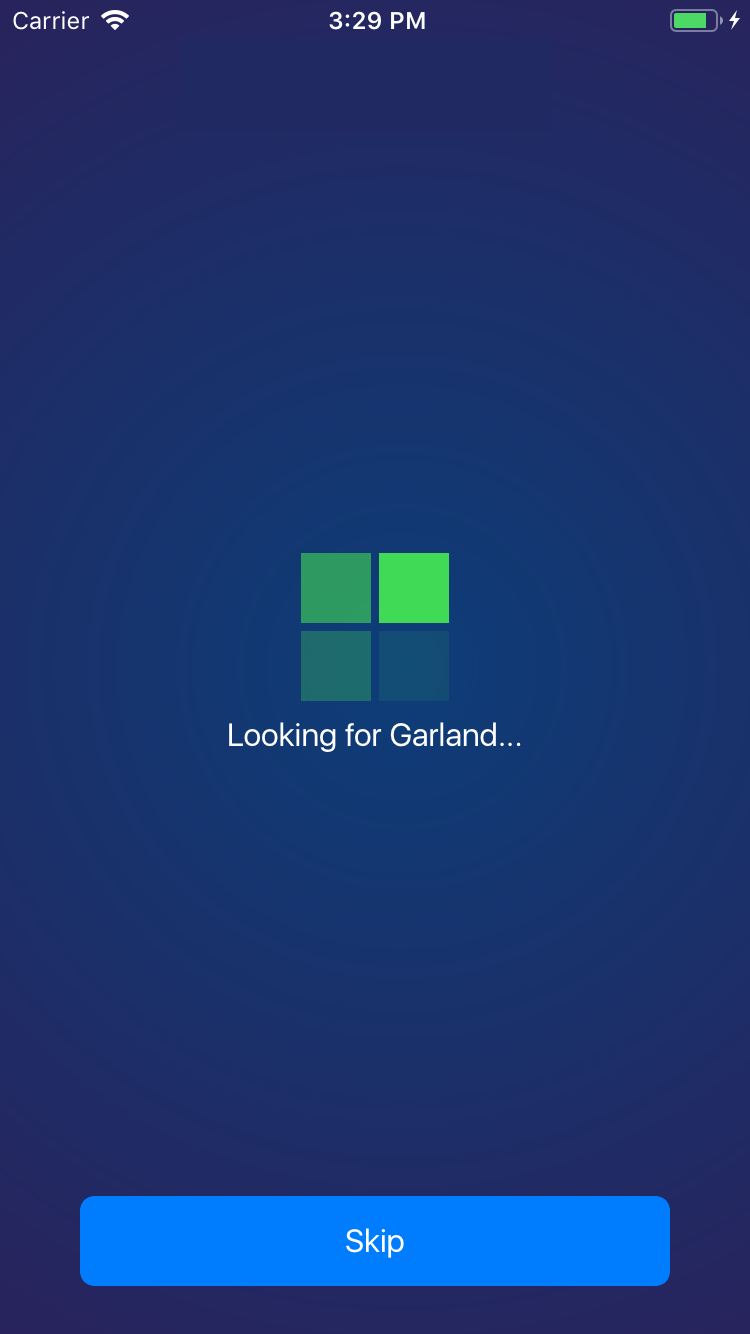
\includegraphics[scale=0.25]{figures/userGuide/loading.png}
	\caption{Экран подключения к гирлянде}
	\label{fig:develop:userGuide:loading}
\end{figure}
~
\begin{figure}[H]
\centering
	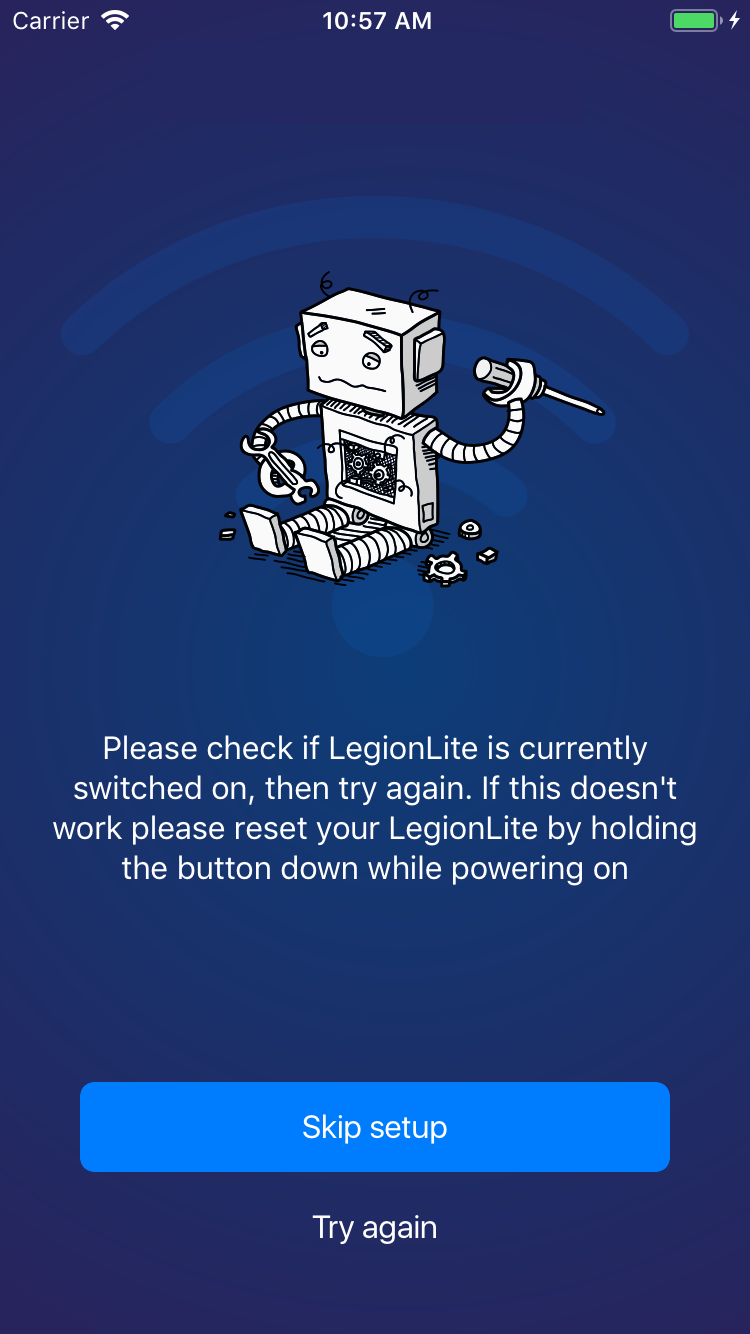
\includegraphics[scale=0.2]{figures/userGuide/failedLoading.png}
	\caption{Экран ошибки подключения к гирлянде}
	\label{fig:develop:userGuide:failedLoading}
\end{figure}
~
\begin{figure}[H]
\centering
	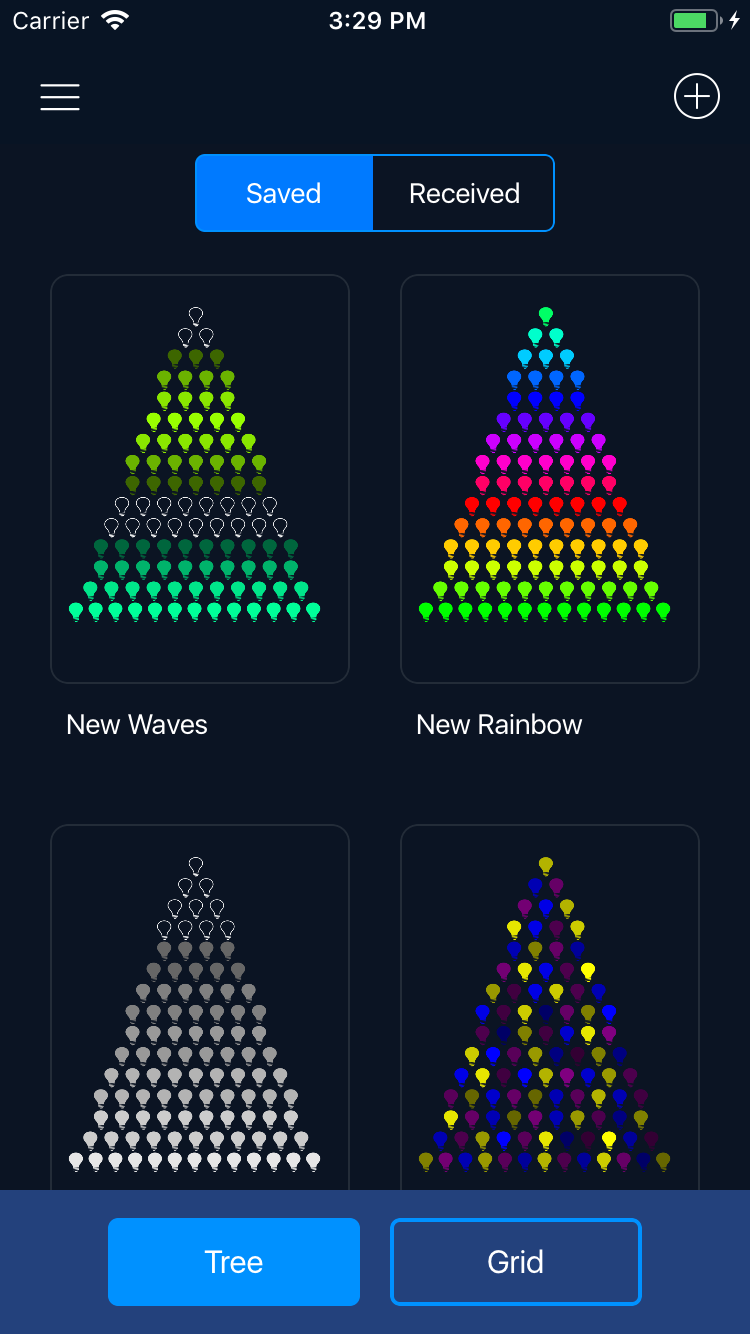
\includegraphics[scale=0.2]{figures/userGuide/mainTree.png}
	\caption{Список всех доступных анимаций для гирлянд типа ``дерево''}
	\label{fig:develop:userGuide:mainTree}
\end{figure}

На главном экране приложения (список всех доступных анимаций), пользователь может выбрать типы просматриваемых доступных анимаций (либо ``Tree'' на рисунке~\ref{fig:develop:userGuide:mainTree}, либо ``Grid'', рисунок~\ref{fig:develop:userGuide:mainGrid}), может создать собственную анимацию по нажатию на кнопку ``+'' (Рисунок~\ref{fig:develop:userGuide:drawingCustom}). Также пользователь, по нажатию на ``гамбургер'', может перейти в меню (Рисунок~\ref{fig:develop:userGuide:sideMenu}). На экране создания собственной анимации пользователь имеет несколько инструментов: точечная кисть (красит по одной лампочке за раз), толстая кисть (красит несколько лампочек за раз) и ластик. Еще пользователь может выбрать нужны цвет с помощью цветового круга (Рисунок~\ref{fig:develop:userGuide:colorPicker}).

~
\begin{figure}[H]
\centering
	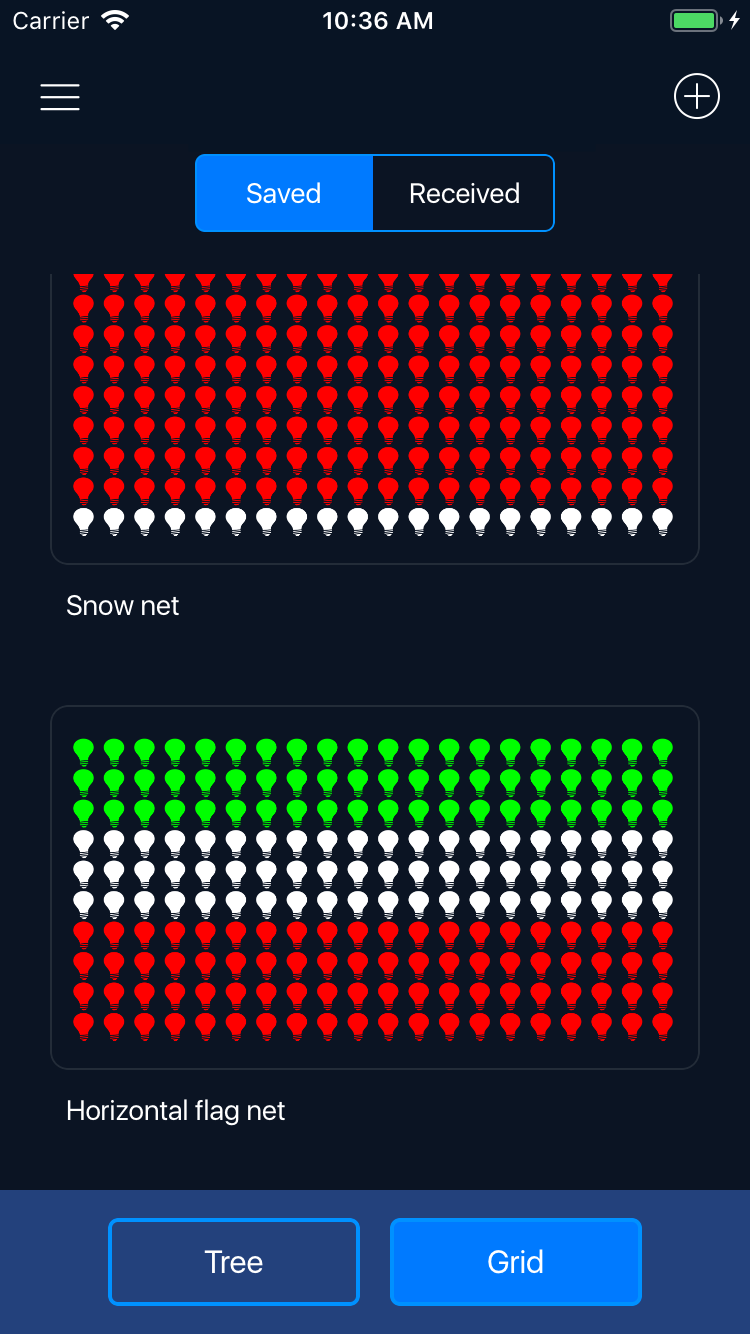
\includegraphics[scale=0.2]{figures/userGuide/mainGrid.png}
	\caption{Список всех доступных анимаций для гирлянд типа ``сетка''}
	\label{fig:develop:userGuide:mainGrid}
\end{figure}
~
\begin{figure}[H]
\centering
	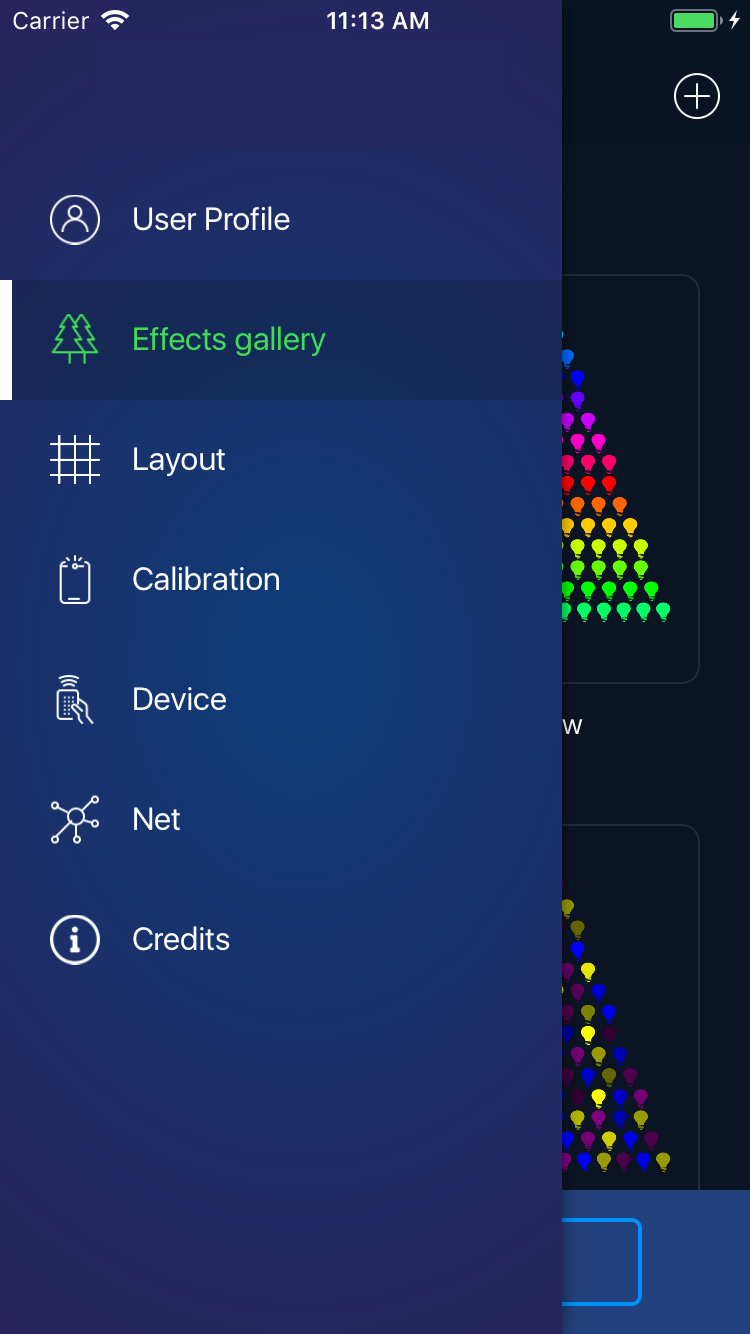
\includegraphics[scale=0.2]{figures/userGuide/sideMenu.png}
	\caption{Меню приложения}
	\label{fig:develop:userGuide:sideMenu}
\end{figure}
~
\begin{figure}[H]
\centering
	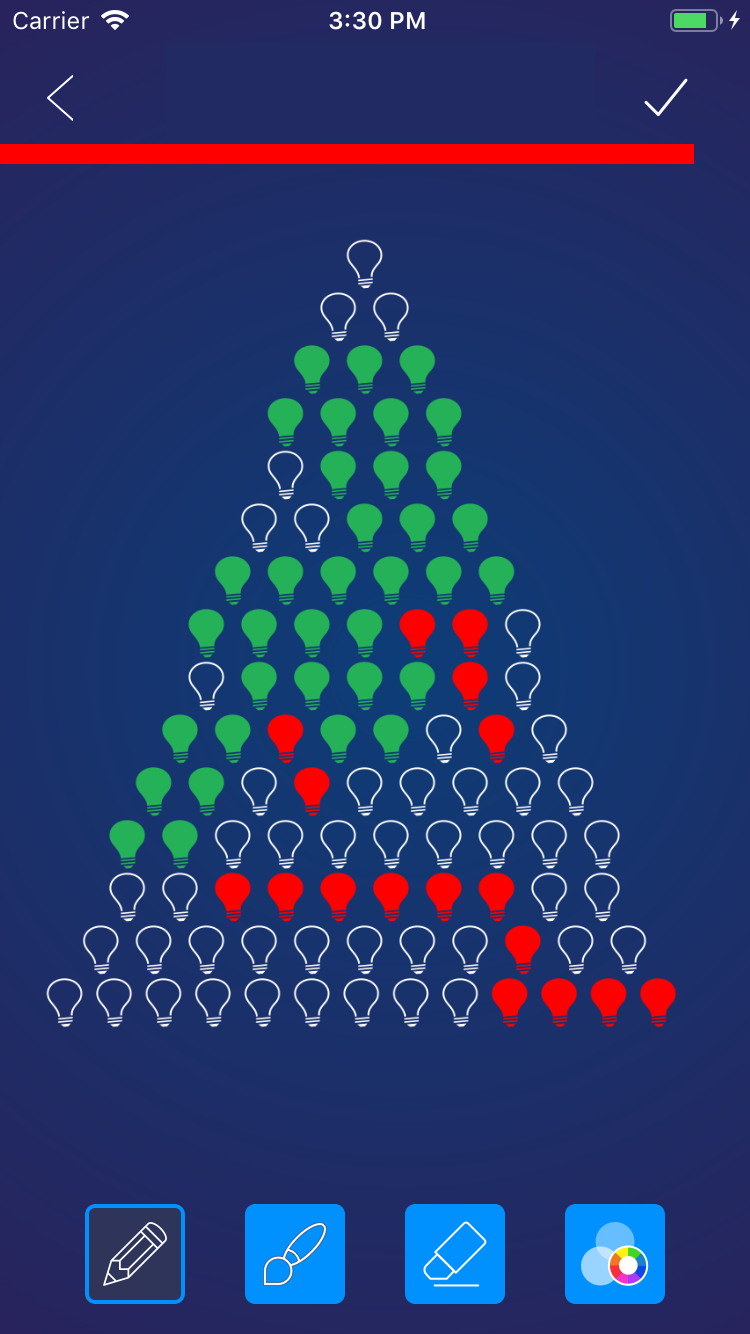
\includegraphics[scale=0.2]{figures/userGuide/drawingCustom.png}
	\caption{Экран создания собственной анимации}
	\label{fig:develop:userGuide:drawingCustom}
\end{figure}
~
\begin{figure}[H]
\centering
	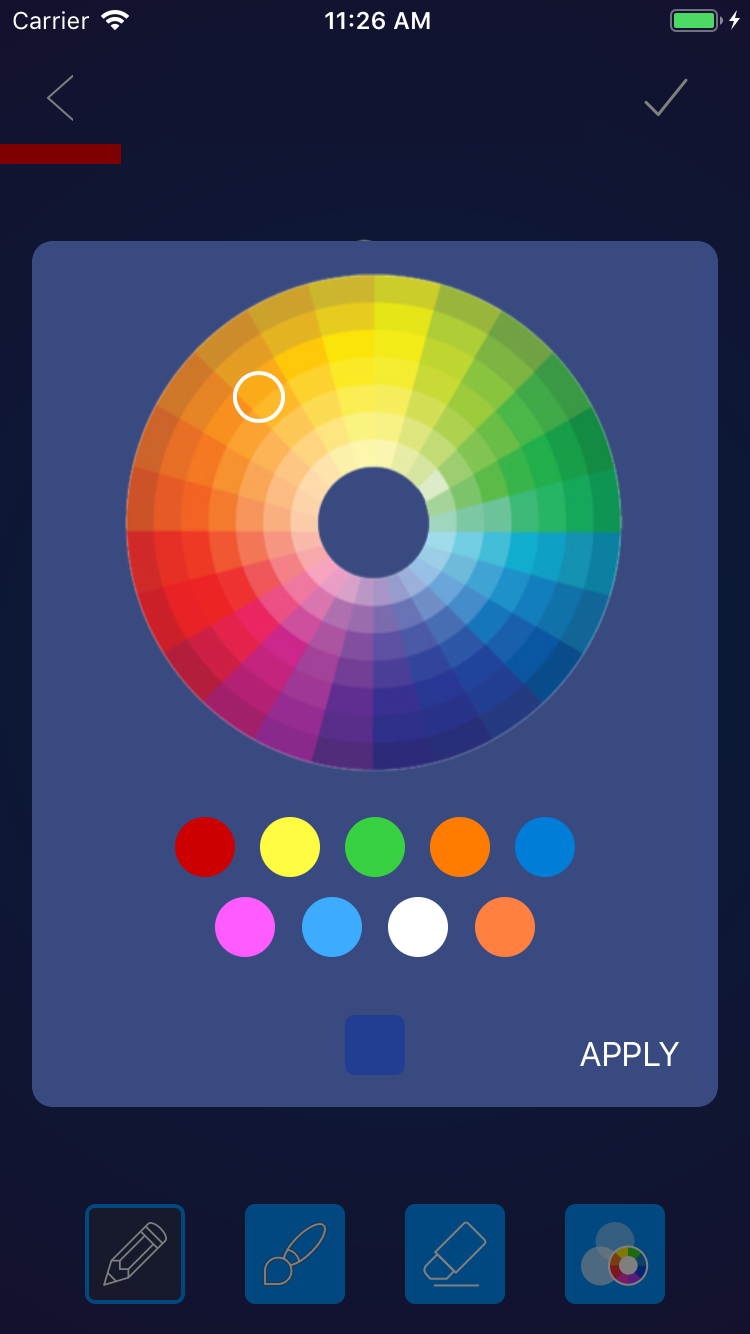
\includegraphics[scale=0.2]{figures/userGuide/colorPicker.png}
	\caption{Экран выбора цвета}
	\label{fig:develop:userGuide:colorPicker}
\end{figure}

При нажатии на анимацию из списка на главном экране, пользователь перейдет на экран просмотра данной анимации (Рисунок~\ref{fig:develop:userGuide:previewDefault}). На данном экране пользователь может отправить анимацию на гирлянду, отправить анимацию другому пользователю, используя его номер телефона (Рисунок~\ref{fig:develop:userGuide:sendingAnimation}), и перейти на экран редактирования анимации. На экране редактирования анимации пользователь, в зависимости от типа анимации может редактировать интенсивность, скорость и набор цветов у анимации (Рисунки~\ref{fig:develop:userGuide:editingNewWaves} и~\ref{fig:develop:userGuide:editingSnake}). Для формирования набора цветов пользователь должен перейти в специальный экран с цветовым кругом (Рисунок~\ref{fig:develop:userGuide:editingColorSequence}).

~
\begin{figure}[H]
\centering
	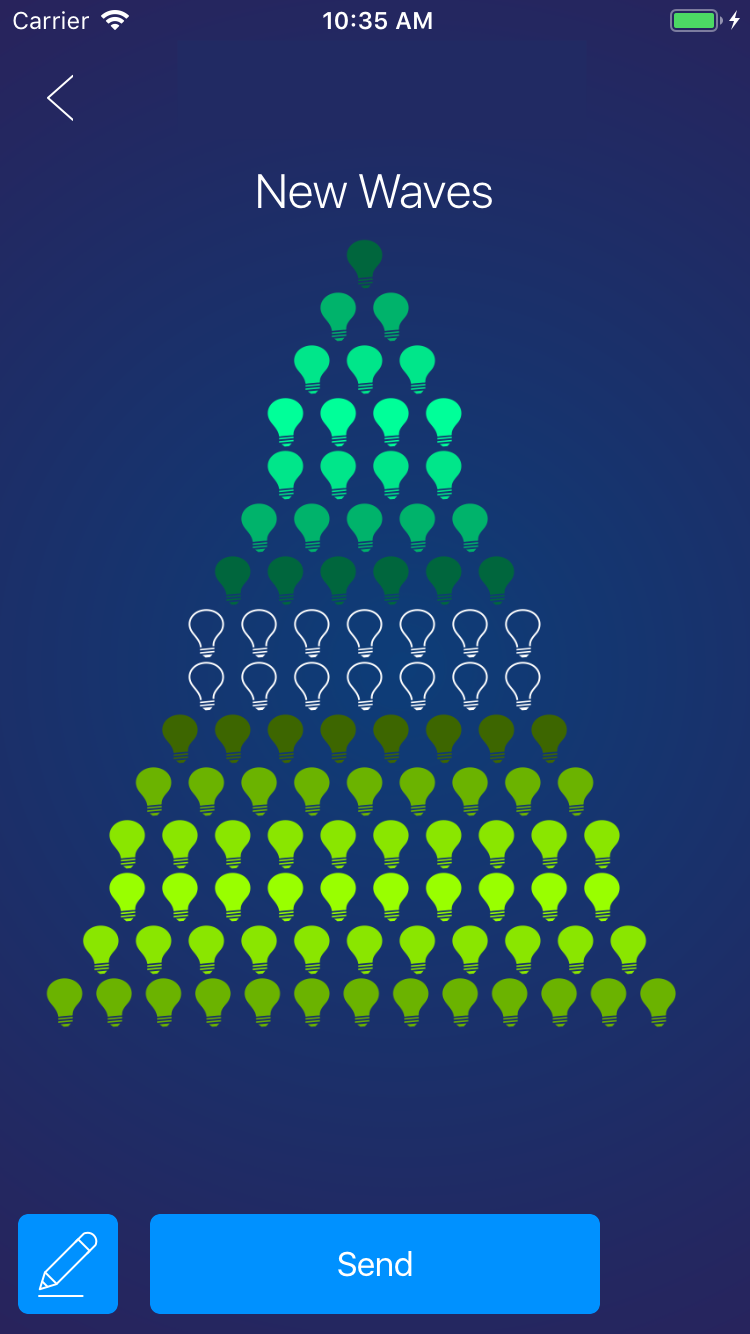
\includegraphics[scale=0.2]{figures/userGuide/previewDefault.png}
	\caption{Экран просмотра существующей анимации}
	\label{fig:develop:userGuide:previewDefault}
\end{figure}
~
\begin{figure}[H]
\centering
	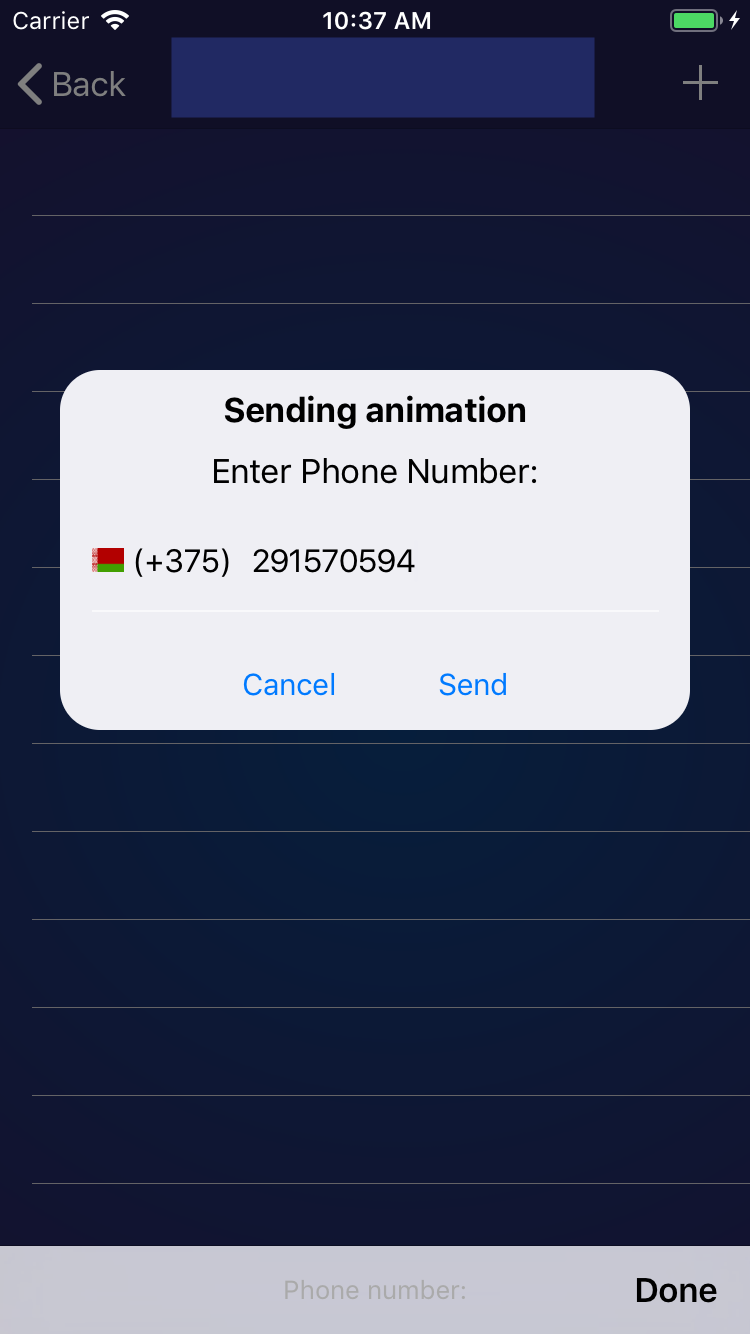
\includegraphics[scale=0.2]{figures/userGuide/sendingAnimation.png}
	\caption{Экран отправки анимации другому пользователю}
	\label{fig:develop:userGuide:sendingAnimation}
\end{figure}
~
\begin{figure}[H]
\centering
	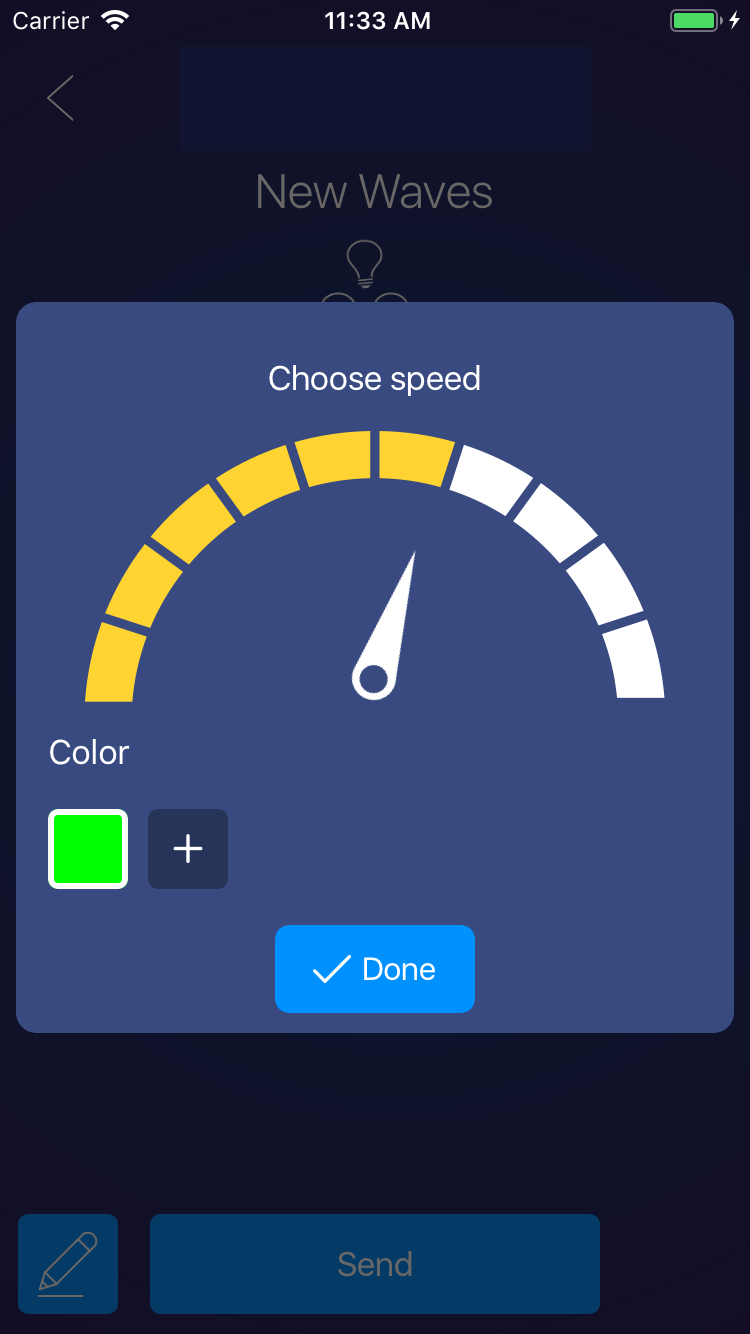
\includegraphics[scale=0.2]{figures/userGuide/editingNewWaves.png}
	\caption{Экран редактирования анимации ``New Waves''}
	\label{fig:develop:userGuide:editingNewWaves}
\end{figure}
~
\begin{figure}[H]
\centering
	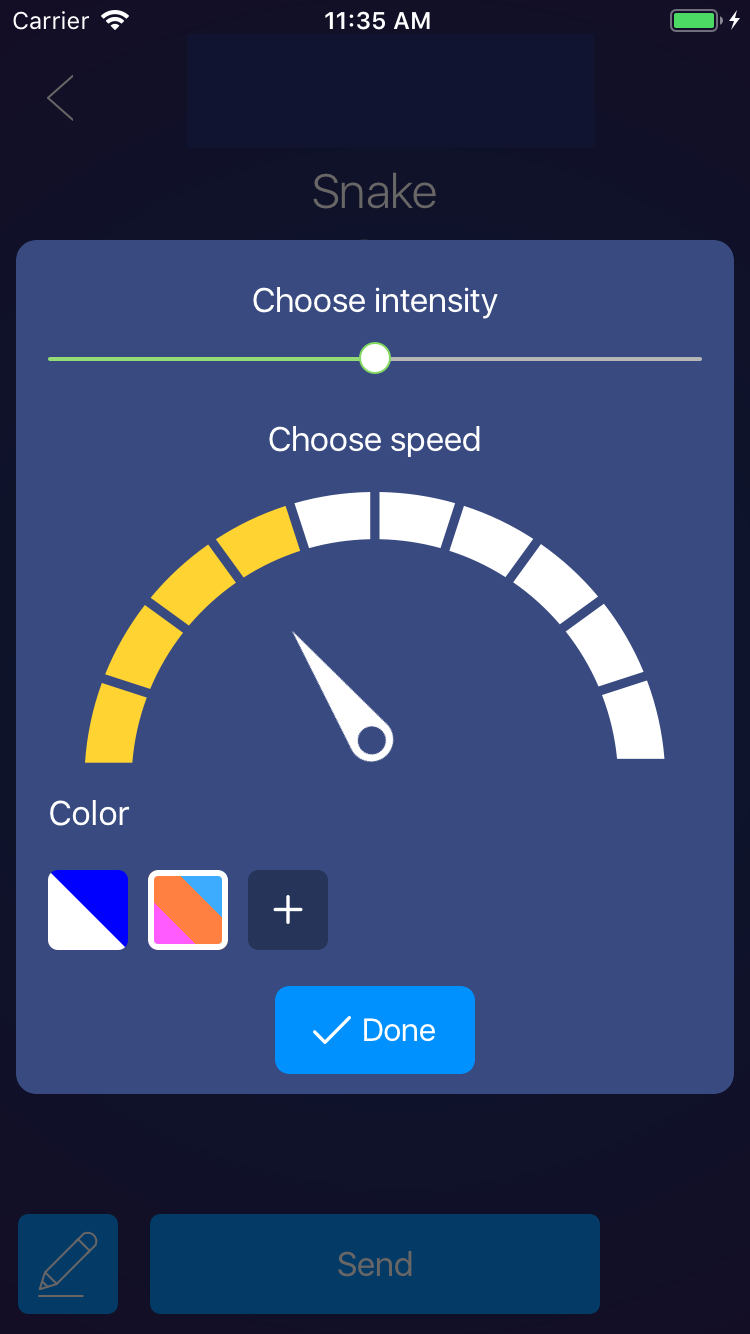
\includegraphics[scale=0.2]{figures/userGuide/editingSnake.png}
	\caption{Экран редактирования анимации ``Snake''}
	\label{fig:develop:userGuide:editingSnake}
\end{figure}
~
\begin{figure}[H]
\centering
	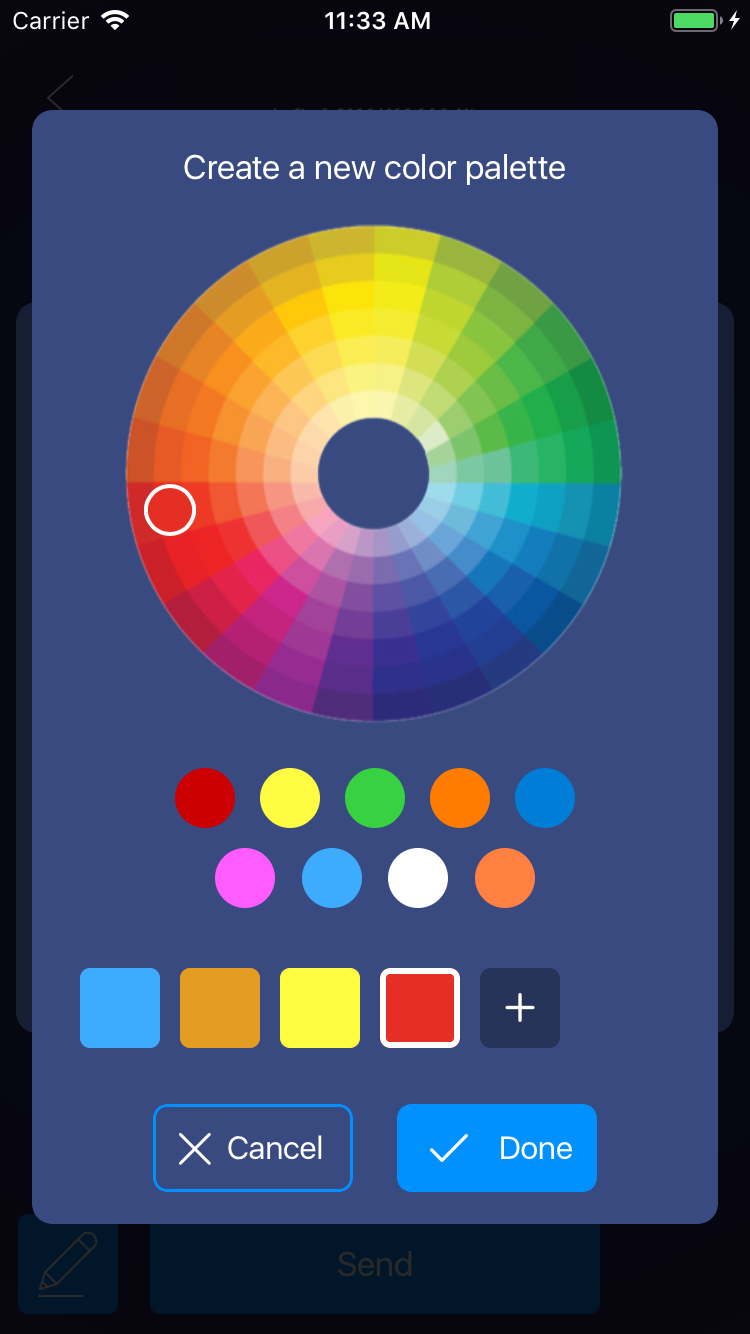
\includegraphics[scale=0.2]{figures/userGuide/editingColorSequence.png}
	\caption{Экран выбора последовательности цветов}
	\label{fig:develop:userGuide:editingColorSequence}
\end{figure}

Чтобы отправить анимацию другому человеку, пользователь должен зайти в свой аккаунт в приложении (Рисунок~\ref{fig:develop:userGuide:signIn}), либо, если у него его еще нет, то зарегистрироваться используя свой номер телефона, электронную почту и пароль (Рисунок~\ref{fig:develop:userGuide:signUp}).

~
\begin{figure}[H]
\centering
	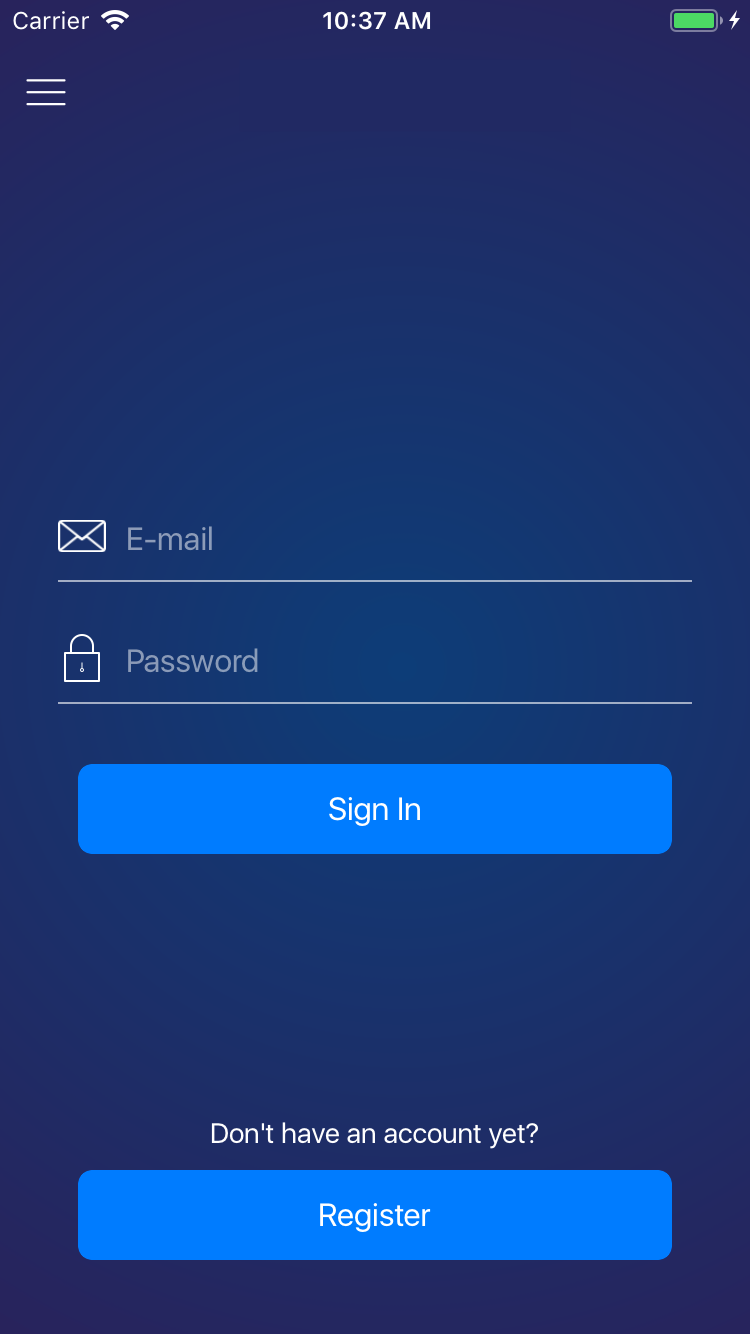
\includegraphics[scale=0.2]{figures/userGuide/signIn.png}
	\caption{Экран входа в аккаунт}
	\label{fig:develop:userGuide:signIn}
\end{figure}
~
\begin{figure}[H]
\centering
	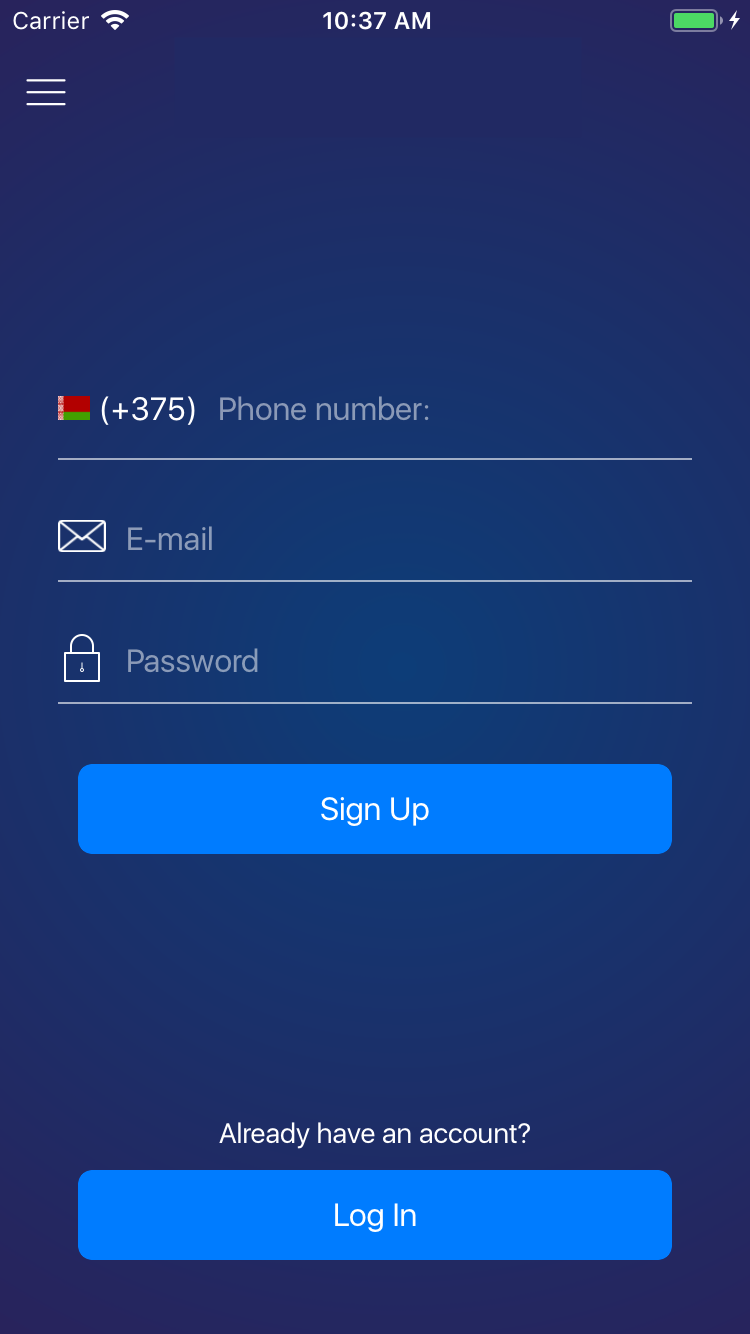
\includegraphics[scale=0.2]{figures/userGuide/signUp.png}
	\caption{Экран регистрации}
	\label{fig:develop:userGuide:signUp}
\end{figure}

Если пользователь подключен к гирлянде напрямую (подключился к ней, как к Wi-Fi точке), то экран ``Устройство'' выглядит как на рисунке~\ref{fig:develop:userGuide:device}. На нем пользователь может подключить ее к существующему Wi-Fi роутеру и просмотреть информацию о гирлянде (ip, mac адреса, версию прошивки, имя гирлянды и т.д.) (Рисунок~\ref{fig:develop:userGuide:device}). Если же пользователь подключен к роутеру, то он будет видеть список доступных гирлянд в этой сети (Рисунок~\ref{fig:develop:userGuide:device}).

~
\begin{figure}[H]
\centering
	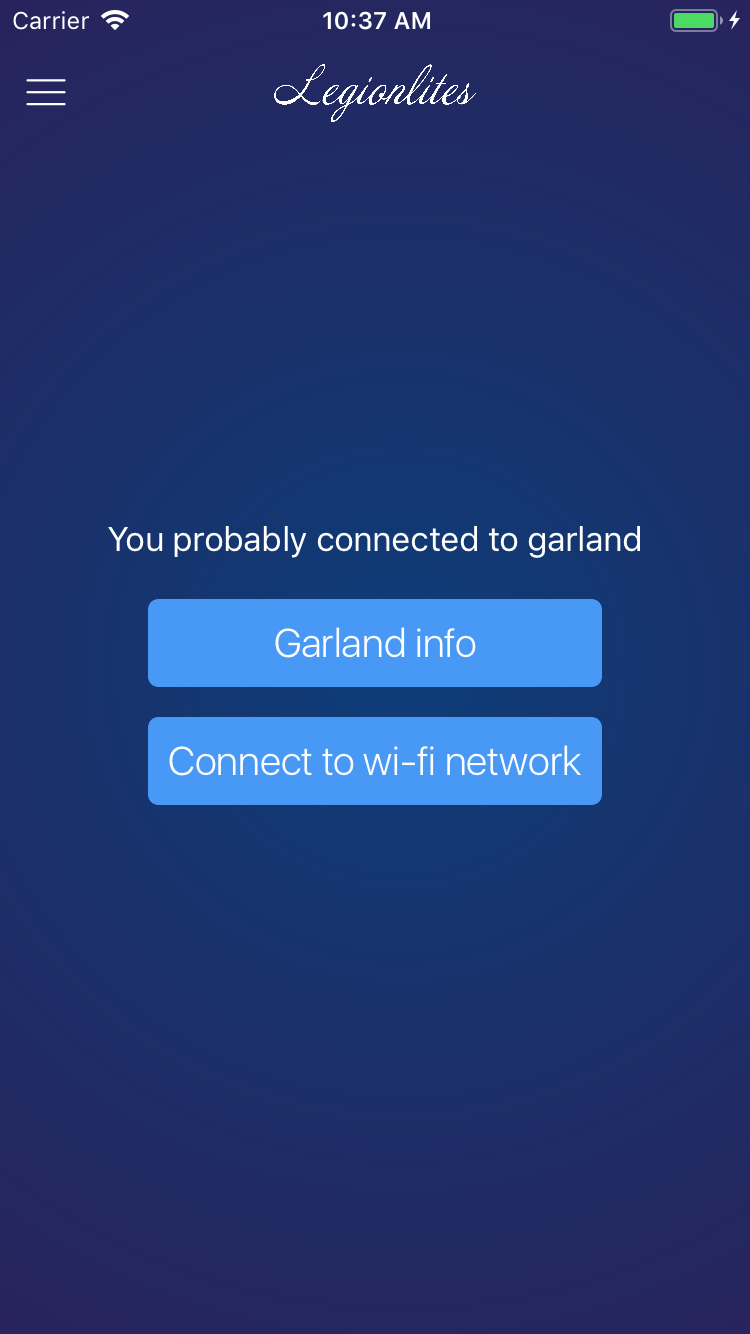
\includegraphics[scale=0.2]{figures/userGuide/device.png}
	\caption{Экран регистрации}
	\label{fig:develop:userGuide:device}
\end{figure}
~
\begin{figure}[H]
\centering
	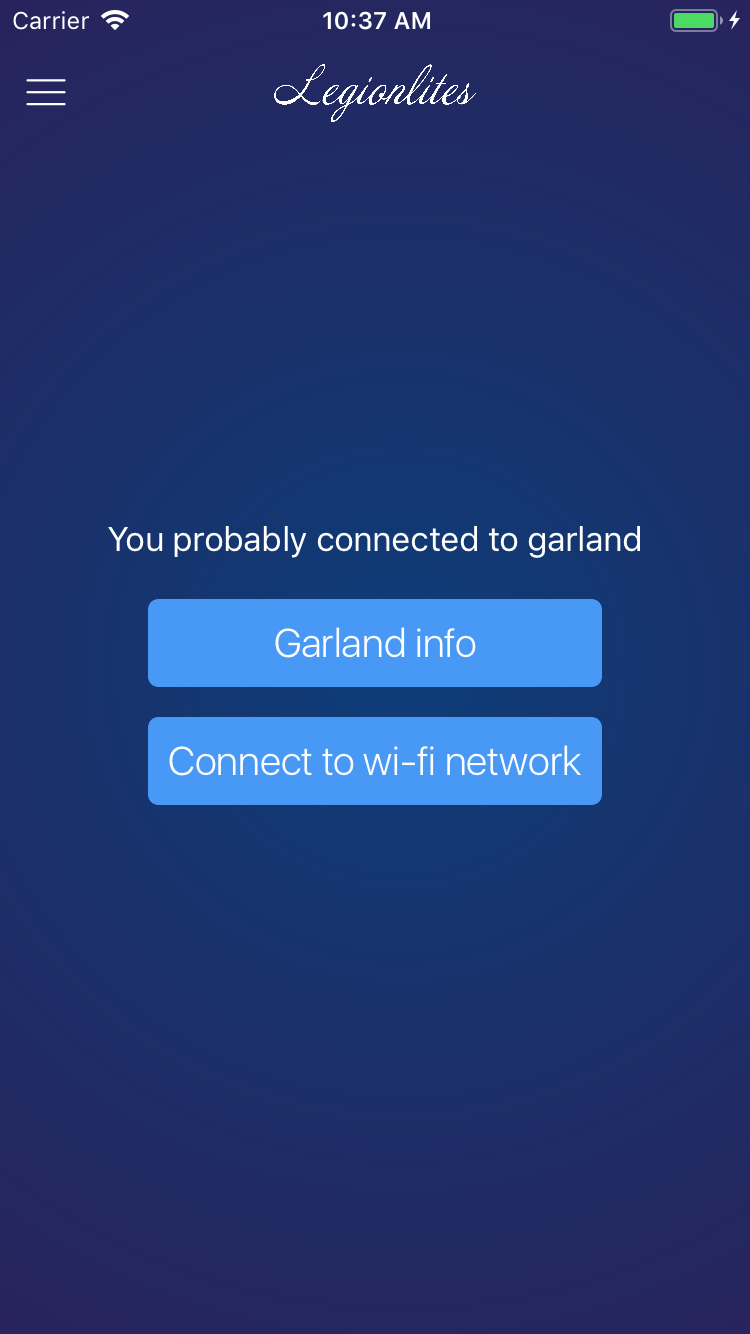
\includegraphics[scale=0.2]{figures/userGuide/device.png}
	\caption{Экран регистрации}
	\label{fig:develop:userGuide:device}
\end{figure}
~
\begin{figure}[H]
\centering
	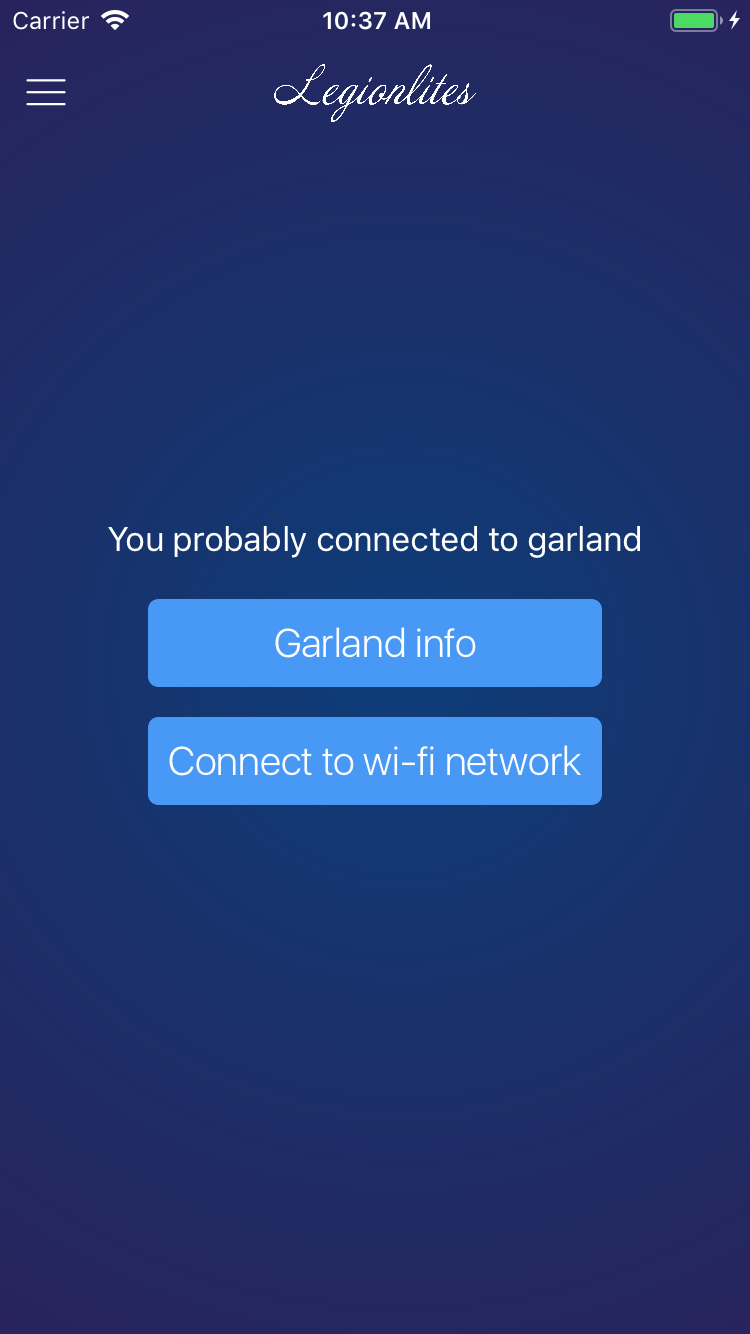
\includegraphics[scale=0.2]{figures/userGuide/device.png}
	\caption{Экран регистрации}
	\label{fig:develop:userGuide:device}
\end{figure}

Для завершения работы с гирляндой пользователю достаточно просто свернуть приложение. Смена анимаций на ней будет доступна через специальную кнопку на самой гирлянде.

